\documentclass{beamer}

\usetheme{Copenhagen}

\title{Cornu Spirals}
\subtitle{From Euler to Ferrari}
\author{Max Mussavian}
\logo{
\includegraphics[height=1.2cm]{Tonbridge_School_logo.png}}
\date[2022]{Arcana, May 2022}
\begin{document}
\begin{frame}[plain]
    \maketitle
\end{frame}
\begin{frame}{Outline}
	\begin{itemize}
		\item History of the Euler Spiral
		\item Definitions: Curves, Lengths and Curvature
		\item Relating the Curve Length to its Curvature
		\item Calculating Fresnel Integrals and the Euler Spiral
		\item Plotting the Euler Spiral and other Fun Curves
		\item Another (Re)discovery: Designing Railways and Roads
	\end{itemize}
\end{frame}

\begin{frame}{History: Bernoulli's Cantilever Problem}
	\begin{itemize}
	\item In 1694 James Bernoulli first studied the Cantilever Problem.
	\item What shape does a thin horizontal beam of negligible mass fixed at one end with weight on the other have?
	\item He called it an \emph{elastica}.
	\item He also posed the converse problem: What shape must a pre-curved beam have in order to be horizontal and straight when a weight is added to the non fixed end?
	\item He claimed $a^2=s R$ where $a$ is constant, $R$ is the radius of curvature and $s$ is arc length (more on this later).
	\end{itemize}
\end{frame}

\begin{frame}{Euler's Solution}
	\begin{columns}
		\begin{column}{0.6\textwidth}
			\begin{itemize}
				\item In 1744 Euler gave the first solution and derived his curve. 
				\item When the curve is horizontal the moment $M$ at any point is equal to the Force $F$ times the distance $s$ from the Force.
				\item From elastic theory the curvature, $\kappa$ at that point is proportional to the moment.
				\item Assuming the curve doesn't stretch the distance from the force is proportional to arc length.
				\item Thus curvature is proportional to the arc length - the Euler Spiral!
			\end{itemize}
		\end{column}
		\begin{column}{0.4\textwidth}
			\begin{figure}[htp]
				\centering
				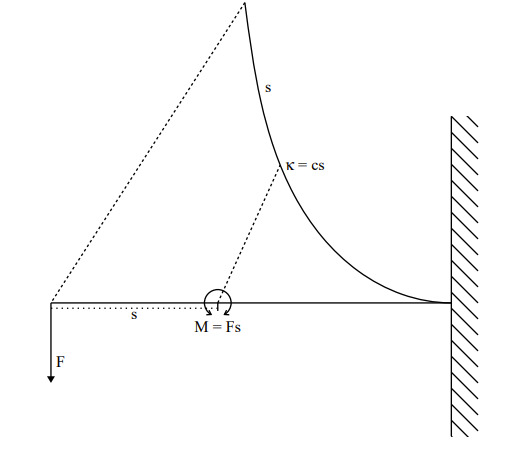
\includegraphics[width=50mm, scale=0.5]{elasticity_problem_Euler_Bernard.png}
			\end{figure}
		\end{column}
	\end{columns}
\end{frame}

\begin{frame}{Euler's Original Spiral}
	\begin{figure}[htp]
		\caption{Reconstruction of Euler's original drawing with spiral superimposed}
		\centering
		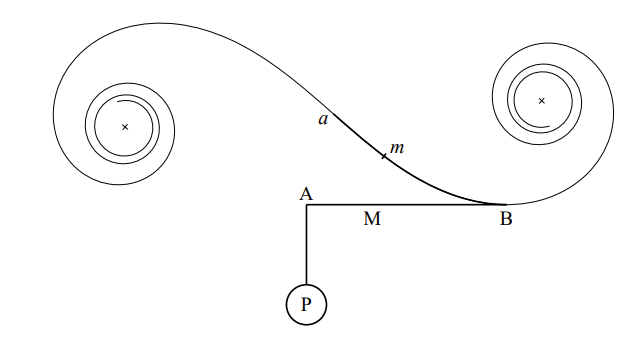
\includegraphics[width=100mm, scale=0.5]{Eulers_original.png}
	\end{figure}..
\end{frame}

\begin{frame}{What is a Curve?}
	Let's define some of the concepts and derive the maths behind the Euler Spiral.
	
		\begin{definition}[A Parametric Curve]
			A parametric curve is a smooth function that has the form
			$x = g(t)$ and $y=h(t)$ defined on an open interval $(a, b)$.
		
			The set of points traced out by the curve is called the trace.
		\end{definition}
		Note that everything we look at here is in 2 dimensions $\mathbb{R}^2$.
	
\end{frame}

\begin{frame}{How Long is a Curve?}
	\begin{definition}[Arc Length]
		The length of a curve $s$ is given by
		$s = \int_{t_1}^{t_2} \sqrt{x'^2+y'^2}dt$
	\end{definition}
	\begin{itemize}
		\item 	The velocity at time $t$ is $\left( \begin{array}{c}
			x'(t)\\
			y'(t)
		\end{array} \right)$ and hence the speed at time $t$ is $\sqrt{x'(t)^2+y'(t)^2}$. Distance travelled (arc length) is the integral of speed with respect to time. 
		
		\item Approximate the trace by line segments. The total length of line segments converges to the arc length as the segments get smaller and smaller.
	\end{itemize}

\end{frame}

\begin{frame}{Some Simple Examples}
\begin{itemize}
	
	\item Circle: We can define a circle with radius $r$ as $x(t)=r \cos(t)$ and $y(t)= r \sin(t)$. The arc length is 
	\[
	s = \int_{0}^{2 \pi} \sqrt{r^2 \sin^2 t + r^2 \cos^2 t}dt = \left[r \right]_{0}^{2 \pi} = 2 \pi r
	\]
	
	\item Parabola: We can define a parabola as $x(t)=t$ and $y(t)=t^2$. The Arc Length between 0 and 1 is 
	\begin{eqnarray*}
	s &=& \int_{0}^{1} \sqrt{1+4t^2}dt \\ &=& \left[\frac{1}{2} t\sqrt{1+ 4 t^2} +\frac{1}{4} \ln \left(2 t+\sqrt{1+ 4 t^2} \right) \right]_{0}^1 \\
	&\approx&	 1.48
	\end{eqnarray*}
\end{itemize}

\end{frame}

\begin{frame}{How Curved is a Curve?}
	The curvature at a point on the curve is the reciprocal of the radius of the circle that approximates the curve.
	\begin{definition}[Curvature]
		The curvature of curve is $\kappa$ given by
		$\kappa=\frac{x' y'' - y' x''}{(x'^2+y'^2)^{3/2}}$
	\end{definition}
	Note: Curvature is signed in two dimensions. Positive curvature corresponds ``bending to the left'' while negative curvature ``bends to the right''.
\end{frame}

\begin{frame}{Explaining Definition for Curvature}
	\begin{columns}
		\begin{column}{0.4\textwidth}
			\begin{figure}
				\centering
				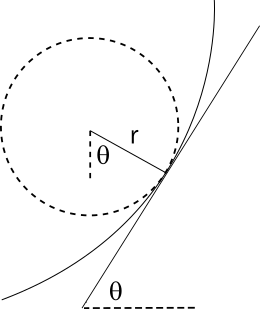
\includegraphics[width=50mm, scale=0.4]{illustration.png}
			\end{figure}
		\end{column}
		\begin{column}{0.6\textwidth}
			\begin{enumerate}
				\item For any circle with radius $r$ we have $s=r \theta$ $\implies$ for ``kissing'' circle 
				$\frac{ds}{dt} = r \frac{d\theta}{dt}$
				
				\item $\frac{ds}{dt} = \sqrt{x'^2+y'^2}$.
				
				\item $\tan \theta = \frac{y'(t)}{x'(t)}$ $\implies$ $\sec ^2 \theta \frac{d\theta}{dt} = \frac{x' y'' - y' x''}{x'^2}$.
				
				\item $\frac{1}{\cos^2 \theta} = \frac{x'^2+y'^2}{x'^2}$ $\implies$
				$\frac{d\theta}{dt}=\frac{x' y'' - y' x''}{x'^2+y'^2}$
				
				
				
				\item Combing gives us
				$r= \frac{ds/dt}{d\theta/dt} =\frac{(x'^2+y'^2)^{3/2}}{x' y'' - y' x''}$
				
				\item Finally $\kappa = \frac{1}{r}$
				
			\end{enumerate}
			
			
			
		\end{column}
	\end{columns}

	
\end{frame}

\begin{frame}{Some Simple Examples}
	\begin{itemize}	
		\item Circle: Recall $x(t)=r \cos(t)$ and $y(t)= r \sin(t)$ 
		\[
		\kappa = \frac{r^2 \sin^2 t + r^2 \cos^2 t}{\left(r^2 \sin^2 t + r^2 \cos^2 t \right) ^ \frac{3}{2}} = \frac{1}{r}
		\]
		
		\item Parabola: Recall $x(t)=t$ and $y(t)=t^2$. 
		
		\[
		\kappa = \frac{2}{\left(1 + 4t^2 \right) ^ \frac{3}{2}}
		\]
	\end{itemize}
\end{frame}

\begin{frame}{Relating Curve Length to Curvature}
	Let's try the following parametrisation for $x$ and $y$
	\begin{eqnarray*}
		x(t) &=& \int_{0}^{t} \cos f(u) du \\
		y(t) &=& \int_{0}^{t} \sin f(u) du
	\end{eqnarray*}
	This gives us
	\begin{eqnarray*}
		x' = x'(t) = \cos f(t) &\mbox{ and }& x''=-f'(t) \sin f(t) \\
		y' = y'(t) = \sin f(t) &\mbox{ and }& y''=f'(t) \cos f(t)
	\end{eqnarray*}
\end{frame}

\begin{frame}{Relating Curve Length to Curvature}
	This gives us the following for slope, arc length and curvature
	\begin{eqnarray*}
	\frac{dy}{dx} &=& \frac{\sin f(t)}{\cos f(t)} = \tan f(t) \\
 	s &=& \int_0^t \sqrt{\cos^2 f(u) + \sin^2 f(u)} du = t \\
 	\kappa &=& \frac{f'(t) \cos^2 f(t) + f'(t) \sin^2 f(t)}{\cos^2 f(t) + \sin^2 f(t)} = f'(t)
 \end{eqnarray*}
\end{frame}

\begin{frame}{Define the Curve by Curve Length and Curvature}
	We can replace the ``time'' variable $t$ by the arc length $s$.
	 
	And the curvature at point $t$ is $f'(t)$. Which means
	 \[
	 f(t) = \int \kappa(t) dt
	 \]
	Thus the equations for the curve become
	\begin{eqnarray*}
	x = x(s) &=& \int_{0}^{s} \cos \left( \int_0^u \kappa(t) dt \right) du \\
	y = y(s) &=& \int_{0}^{s} \sin \left( \int_0^u \kappa(t) dt \right) du
	\end{eqnarray*}
	Hence the curve is defined by arc length and curvature alone.
\end{frame}

\begin{frame}{A Very Simple Example}
	We can make the curvature $\kappa$ constant and equal to 1. Then 
	$ \int_0^u \kappa(t) dt = u $ and
	\begin{eqnarray*}
		x = x(s) &=& \int_{0}^{s} \cos u du = \sin s\\
		y = y(s) &=& \int_{0}^{s} \sin u du = - \cos s + 1
	\end{eqnarray*}
	which is the parametric curve for a circle with centre $(0, 1)$ and radius $1$.
	
\end{frame}


\begin{frame}{The Euler Spiral}
	Recall: Euler defined his curve as one where the curvature is proportional to arc length.
	
	\begin{center}
		\boxed{\kappa(s) = s}
	\end{center}
	Then 
	$ \int_0^u \kappa(t) dt = \frac{u^2}{2} $ and
	\begin{eqnarray*}
		x = x(s) &=& \int_{0}^{s} \cos \frac{u^2}{2} du\\
		y = y(s) &=& \int_{0}^{s} \sin \frac{u^2}{2} du
	\end{eqnarray*}

	But since these integrals can't be solved analytically how were they calculated?
\end{frame}

\begin{frame}{Solving the Integrals: Euler}
	\begin{itemize}
		\item In 1744 Euler derived these integrals.
		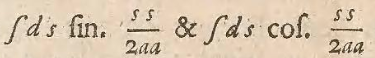
\includegraphics[width=50mm, scale=0.5]{euler_scripture_1.png}	
		\item He derived a series expansion which is still a viable method for small $s$.
		
		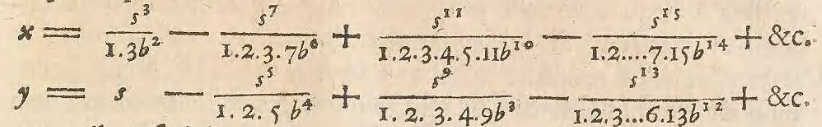
\includegraphics[width=100mm, scale=0.7]{euler_scripture.png}
		
		\item In 1781 he proved the integrals for limits between 0 and $\infty$ are equal to  $\frac{a \sqrt{\pi}}{2}$ 
	\end{itemize}
\end{frame}

\begin{frame}{Solving integrals: Fresnel and Cornu}
	\begin{itemize}
		\item In 1818 Augustin Fresnel rediscovered these integrals when he investigated the diffraction of light through a slit. He showed that the intensity (under some assumptions) was 
		\[
		\left( \int_{0}^{s}\cos \left( \pi t^2 / 2 \right) dt \right) ^2 + 
		\left( \int_{0}^{s}\sin \left( \pi t^2 / 2 \right) dt \right) ^2
		\] 
		\item Up to a factor of $\pi$ the integrals are the same as the ones Euler derived.
		\item These integrals are now called the \emph{Fresnel Integrals}.
		\item Fresnel calculated them for values of $s$ between 0.1 and 5.1.
		\item In 1874 Alfred Cornu calculated values and plotted the Euler spiral accurately. Hence the Euler spiral is also known as a Cornu spiral.
	\end{itemize}
\end{frame}


\begin{frame}{Making a Plotter in Python}
	\begin{columns}
		\begin{column}{0.5\textwidth}
			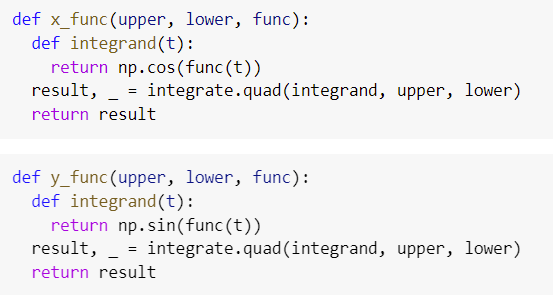
\includegraphics[width=50mm, scale=0.5]{code_1.png}
			
			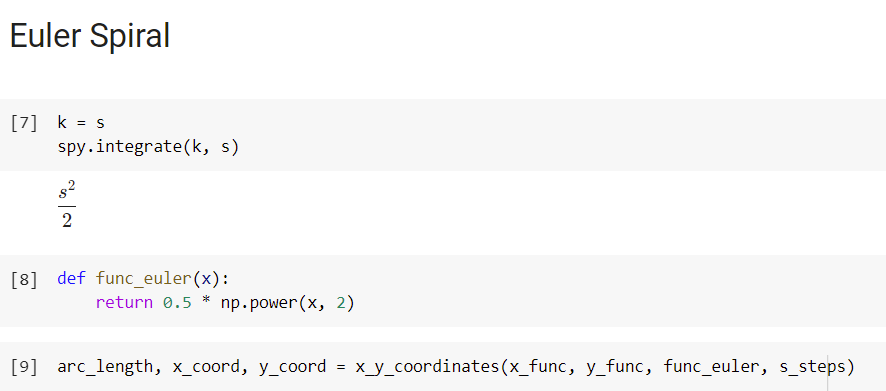
\includegraphics[width=50mm, scale=0.5]{code_2.png}
		\end{column}
		\begin{column}{0.5\textwidth}
		Now we can use computers and numerical methods to evaluate these integrals.
			
		\end{column}
	\end{columns}
\end{frame}


\begin{frame}{The Euler Spiral}
	\begin{figure}
		\caption{The Euler Spiral aka Cornu Curve}
		\centering
		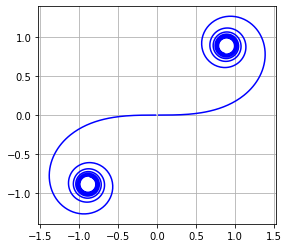
\includegraphics[width=70mm, scale=0.5]{euler_spiral.png}
	\end{figure}
	
\end{frame}

\begin{frame}{The Euler Spiral - $x$ $y$ Coordinates}
	\begin{figure}
	\caption{Fresnel Integrals with arguments $\frac{u^2}{2}$}
	\centering
	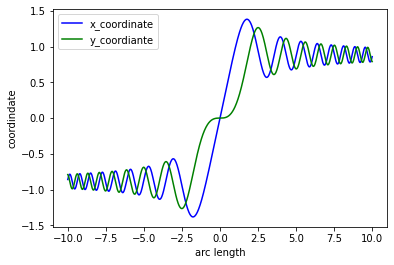
\includegraphics[width=70mm, scale=0.5]{euler_x_vs_y.png}
	\end{figure}
	These converge to $\pm \frac{\sqrt{\pi}}{2} \approx 0.8862$.
\end{frame}

\begin{frame}{Other Fun Curves: Even Powers of $s$}
	\begin{figure}
		\caption{$\kappa(s) = s^2$}
		\centering
		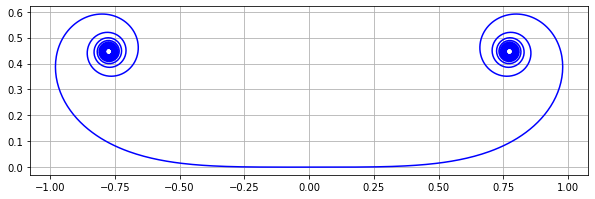
\includegraphics[width=85mm, scale=0.5]{chaise_longue.png}
	\end{figure}
\end{frame}

\begin{frame}{More Fun Curves: Mix in a Bit of a Circle}
	\begin{figure}
		\caption{$\kappa(s) = s ^ 2 -2.19$}
		\centering
		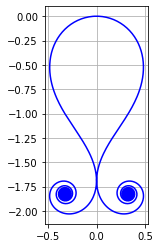
\includegraphics[width=35mm, scale=0.2]{s_squared_minus_219.png}
	\end{figure}
\end{frame}

\begin{frame}{More Fun Curves: Polynomials}
	\begin{figure}
		\caption{$\kappa(s) = 5 s ^ 4 - 18 s ^ 2 + 5$}
		\centering
		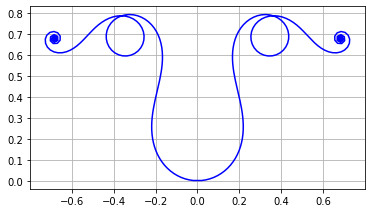
\includegraphics[width=70mm, scale=0.5]{five_s^4.png}
	\end{figure}
\end{frame}

\begin{frame}{More Fun Curves: Trigonometric Functions}
	\begin{figure}
		\caption{$\kappa(s) = \cos(s) - s \sin(s)$}
		\centering
		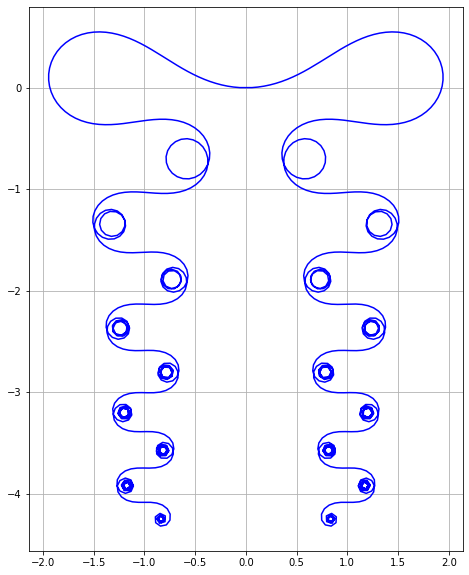
\includegraphics[width=50mm, scale=0.2]{elegant_madness.png}
	\end{figure}
\end{frame}
	
\begin{frame}{More Fun Curves: Hyperbolic Functions}
	\begin{figure}
		\caption{$\kappa(s) = \sinh(s) - 5.19$}
		\centering
		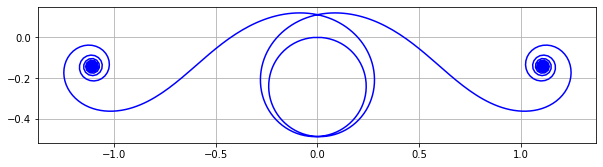
\includegraphics[width=100mm, scale=0.5]{sinh.png}
	\end{figure}
\end{frame}

\begin{frame}{Another (Re)discovery of the Euler Spiral}
	\begin{itemize}
		\item As trains became faster in the 19th century, the Euler spiral was rediscovered by railway designers.
	\end{itemize}
\end{frame}

\begin{frame}{Designing Roads and Railways}
	\begin{enumerate}
		\item Transition curves are used to link straight sections of motorways or railways.
		\item They are designed to give passengers a smooth ride.
		\item In particular so sudden changes in acceleration.

	\end{enumerate}
		\begin{figure}
		\caption{Cloverleaf Motorway Interchange}
		\centering
		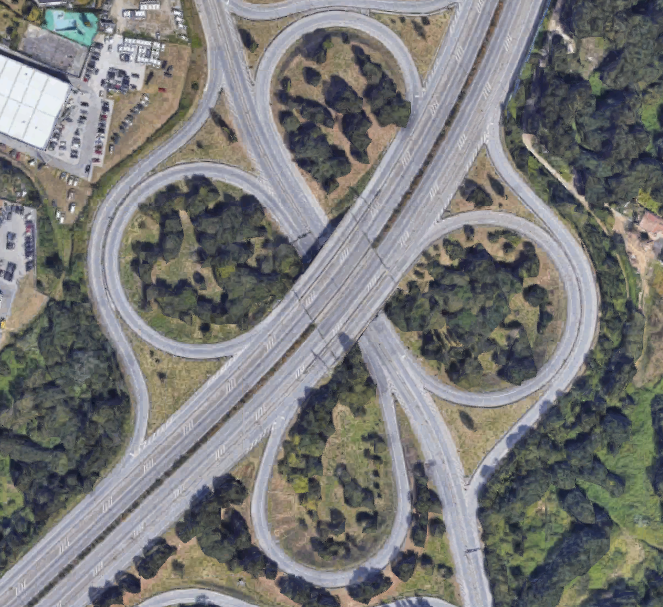
\includegraphics[width=20mm, scale=0.5]{cloverleaf_motorway.png}
	\end{figure}

\end{frame}

\begin{frame}{Why Transition Curves are Euler Spirals}
	\begin{itemize}
	\item The acceleration along the transition curve is given by
 	 \[
 	 a=s''(t) \vec{T}+\kappa s'(t)^2 \vec{N}
 	 \]
 	 Where $\vec{T}$ is the unit tangent vector and $\vec{N}$ is the unit normal vector.
 	 \item If the car/train is going round the curve at constant speed $s'(t)=constant$ and $s''(t)=0$.	
 	 \item The acceleration at constant speed only depends on the curvature $\kappa$ and speed $s'(t)$ in the direction of the normal vector.
	\end{itemize}
\end{frame}

\begin{frame}{Case 1: Semicircular Curves}
	A closed  track is made up of four segments.
	\begin{enumerate}
		\item A straight track of length 1km
		\item A semicircular track of length 1km. This has radius $1,000 / \pi m \approx 318.31m$
		\item A straight track of length 1km
		\item A semicircular track of length 1km.
	\end{enumerate}
	Let the vehicle go around the track at a constant speed of $60 km/h = 16 \frac{2}{3} m/s$.
\end{frame}

\begin{frame}{Case 1: Position and Acceleration}
	\begin{columns}
		\begin{column}{0.8\textwidth}			
			\begin{figure}
				\caption{Position and Acceleration}
				\centering
				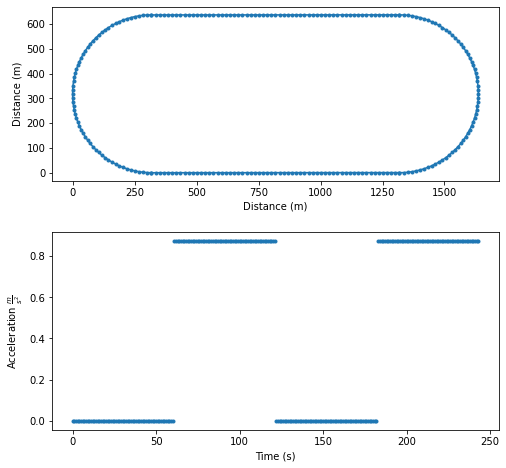
\includegraphics[width=70mm, scale=0.2]{circular_track.png}
			\end{figure}
		\end{column}
		\begin{column}{0.33\textwidth}
			Note: The acceleration is a step function. 
			
			
			As a passenger you would feed the full centrifugal force pushing you outward the moment you entered the curve.			
		\end{column}
	\end{columns}
\end{frame}


\begin{frame}{Case 2: Euler Spiral Transition Curves}
	\begin{itemize}
		\item A closed track with same width and height. 
		\item Replace semicircles with two parts of an Euler Spiral.
		\item Recall that the curvature is proportional to arc length. $\kappa = \alpha s $ for some $\alpha$.
		\item The width and height of an Euler Spiral that turns through $\pi/2$ is given by 
		\begin{eqnarray*}
			width &=& \sqrt{\pi / \alpha} C(1) \\
			height &=& \sqrt{\pi /\alpha}S(1)
		\end{eqnarray*}
		where $S(z)=\int_{0}^{z}\sin \left( \pi t^2 / 2 \right) dt$ and $C(z)=\int_{0}^{z}\sin \left( \pi t^2 / 2 \right) dt$  is the standard Fresnel integrals.
	
	\end{itemize}
	
	\[
	\alpha = \frac{\pi S(1)^2}{r^2} \approx 5.95 \times 10 ^{-6}
	\]
	
\end{frame}

\begin{frame}{Case 2: Euler Spiral Transition Curves}
	\begin{columns}
		\begin{column}{0.8\textwidth}			
			\begin{figure}
				\caption{Position and Acceleration}
				\centering
				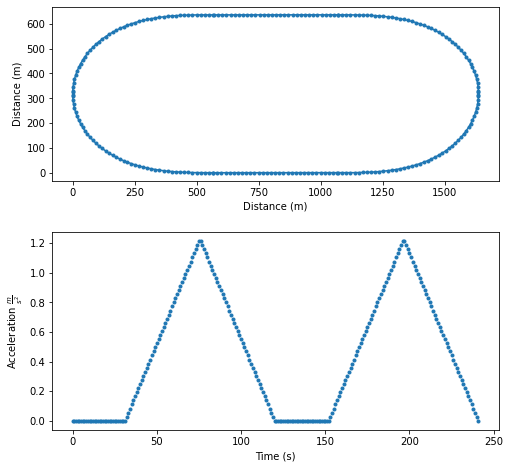
\includegraphics[width=70mm, scale=0.2]{euler_track.png}
			\end{figure}
		\end{column}
		\begin{column}{0.33\textwidth}
			Note: The acceleration is a increases linearly as we move through the curve.
			
			The maximum acceleration however at the apex is greater than with the semicircular track. 
					
		\end{column}
	\end{columns}

\end{frame}

\begin{frame}{Case 1 vs Case 2}
	\begin{figure}
		\caption{Curves Compared}
		\centering
		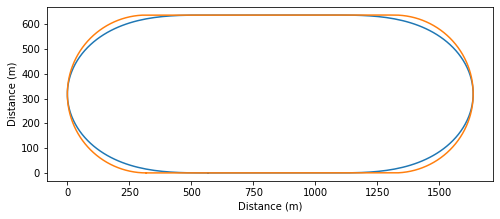
\includegraphics[width=70mm, scale=0.2]{circular_vs_euler_track.png}
	\end{figure}
	
\end{frame}

\begin{frame}
	
\end{frame}
\end{document}
